\documentclass[a4paper, 10pt]{article}
\usepackage[top=2cm, bottom=3cm, left = 2cm, right = 2cm]{geometry} 
\geometry{a4paper} 
\usepackage{textcomp}
\usepackage{graphicx} 
\usepackage{amsmath,amssymb}  
\usepackage{bm}  
\usepackage{memhfixc} 
\usepackage{fancyhdr}
\usepackage{enumerate}
\usepackage{tikz}
\usepackage{float}
\usepackage{booktabs}
\usepackage{listings}
\usepackage[framed]{ntheorem}
\pagestyle{fancy}
\setlength{\headheight}{14pt}
\addtolength{\topmargin}{-2pt}
\theoremstyle{nonumberplain}


\title{Design and Implementation of a Bandwidth
Controlled Shared Memory Communication Model for Edge and Cloud Containers}

\author{Hossein Afkar \and Sina MirSattarian}
%\date{}

\begin{document}
\maketitle
% \tableofcontents

\section{Introduction}
Container communication plays an important role in cloud and edge containers
ecosystem. In order to utilize the vast capabilities of the containers in the
real-time world and industry 4.0 we need to add real-time capabilities to the
container scheduling and communications. Also in mixed-criticality concepts it
is important to isolate the effects of a malfunctioning container on other
containers that are working in their normal or high priority modes. In order
to achieve that we tried to design and implement a communication system based
on the shared memory model. We choose the shared memory model because of its
potential in achieving high performance and throughput levels. Our design in
based on local communication in shared memory host. Local communication is
an important part of the containers world and pipelines. Achieving a good
and real-time local communication model can enable us to bring the features of
containrization such as isolation and ease of delivery to the real-time world.
Also it is a step forward in achieving a real-time hypervisor for containers in
real-time world. Ideas related to this section was collected from the
\cite{survey}.
\section{Design and Implementation}
In this section, we will discuss the design and implementation of a
bandwidth-controlled shared memory channel for container communication.
Our design goals are stated as follows:
\begin{itemize}
    \item Control Bandwidth of the memory
    \item Reserve and repurpose unused bandwidth
    \item Achieve performance isolation
    \item Bound the latency of the communications using lock less containers
\end{itemize}
To control the bandwidth we used the MemGuard paper \cite{memguard}.
This paper used the performance counters of the intel processor to determine
the read and write access for a physical core in the system. We need to
implement this for a memory region. \\
Performance counters do not provide us with the tracing information of accesses
to specific memory regions therefore we need to ask either the kernel or
user to bookkeep for the size of the memory access. User is a better
choice for performance reasons. So our approach is allocating a budget to each
shared memory region and supplying the user with a library for read and write
purposes. Before every read and write the user will update the bookkeeping
associated with the shared memory region. Also, the budget will be reset on
the hyperperiod specified by the real-time system designer. \\
The next goal is to preserve and repurpose the bandwidth. This is done by
predicting the next hyperperiod bandwidth usage. This is done using
the exponentially weighted moving average. If our prediction is lower than
the static budget, it will be added to the global bandwidth budget. If a process
needs a budget it can ask the global bandwidth budget for additional budget.
The exact algorithm on how this works can be found in the MemGuard \cite{memguard}
paper. \\
Achieving performance isolation in memory is done by bounding the bandwidth.
By bounding the bandwidth we can be sure that no bad or malfunctioning
container creates contention on the system bus and deprive other containers
from using their share of the memory. \\
Bounding the latency can be done using unix signals and
\textit{CLOCK\_THREAD\_CPUTIME\_ID}. If the need arises for such control on
memory we can use it to cancel a read or write function call. This method is
almost unnecessary because most real-time systems designers calculate WCET and
are aware of the communications overhead. \\
Our proposed design is using new kernel system calls to handle creating the
shared memory. Also, shared memory is segmented using a lockless data structure
that eases the uses of mutexes which are bad for real-time scheduling problems.

\begin{figure}[H]
    \centering
    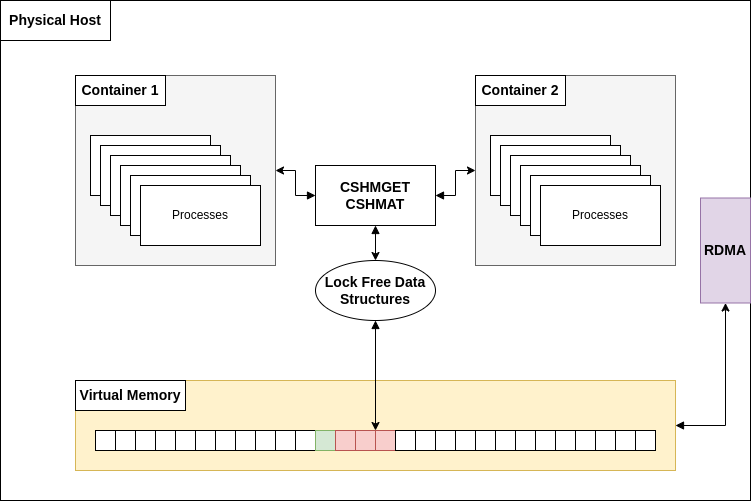
\includegraphics[scale=0.3]{dist.png}
    \caption{Our proposed design}
\end{figure}

Our Implementation revolves around the linux kernel and user level libraries.
In order to get shared memory spaces we devised and edited linux kernel
and added a number of 3 syscalls that create and map the address to the
virtual address space of the process. In order to synchronize the shared memory
between containers we used an atomic vector implementation described in the
\cite{vector}. We implemented the algorithms described in this vector using
compare and swap primitives in the hardware. By having a lock free
implementation of a synchronized data structure we can be sure that issues
regarding mutexes like priority inversion and hard program verification is
solved in our implementation. \\
Then two programs are written to handle our design goals. One program is a user
level client that is supplied with a user level bookkeeping library and our
lock free vector implementation. The other is a server that handles global
budget allocation and hyperperiod refreshes. \\
Our results show that the budget is allocated justly and the programs work as
intended. Unfortunately we could not devise test cases in the allocated
project deadline to show isolation in presence of a malfunctioning or
bad container.

\begin{figure}[H]
    \centering
    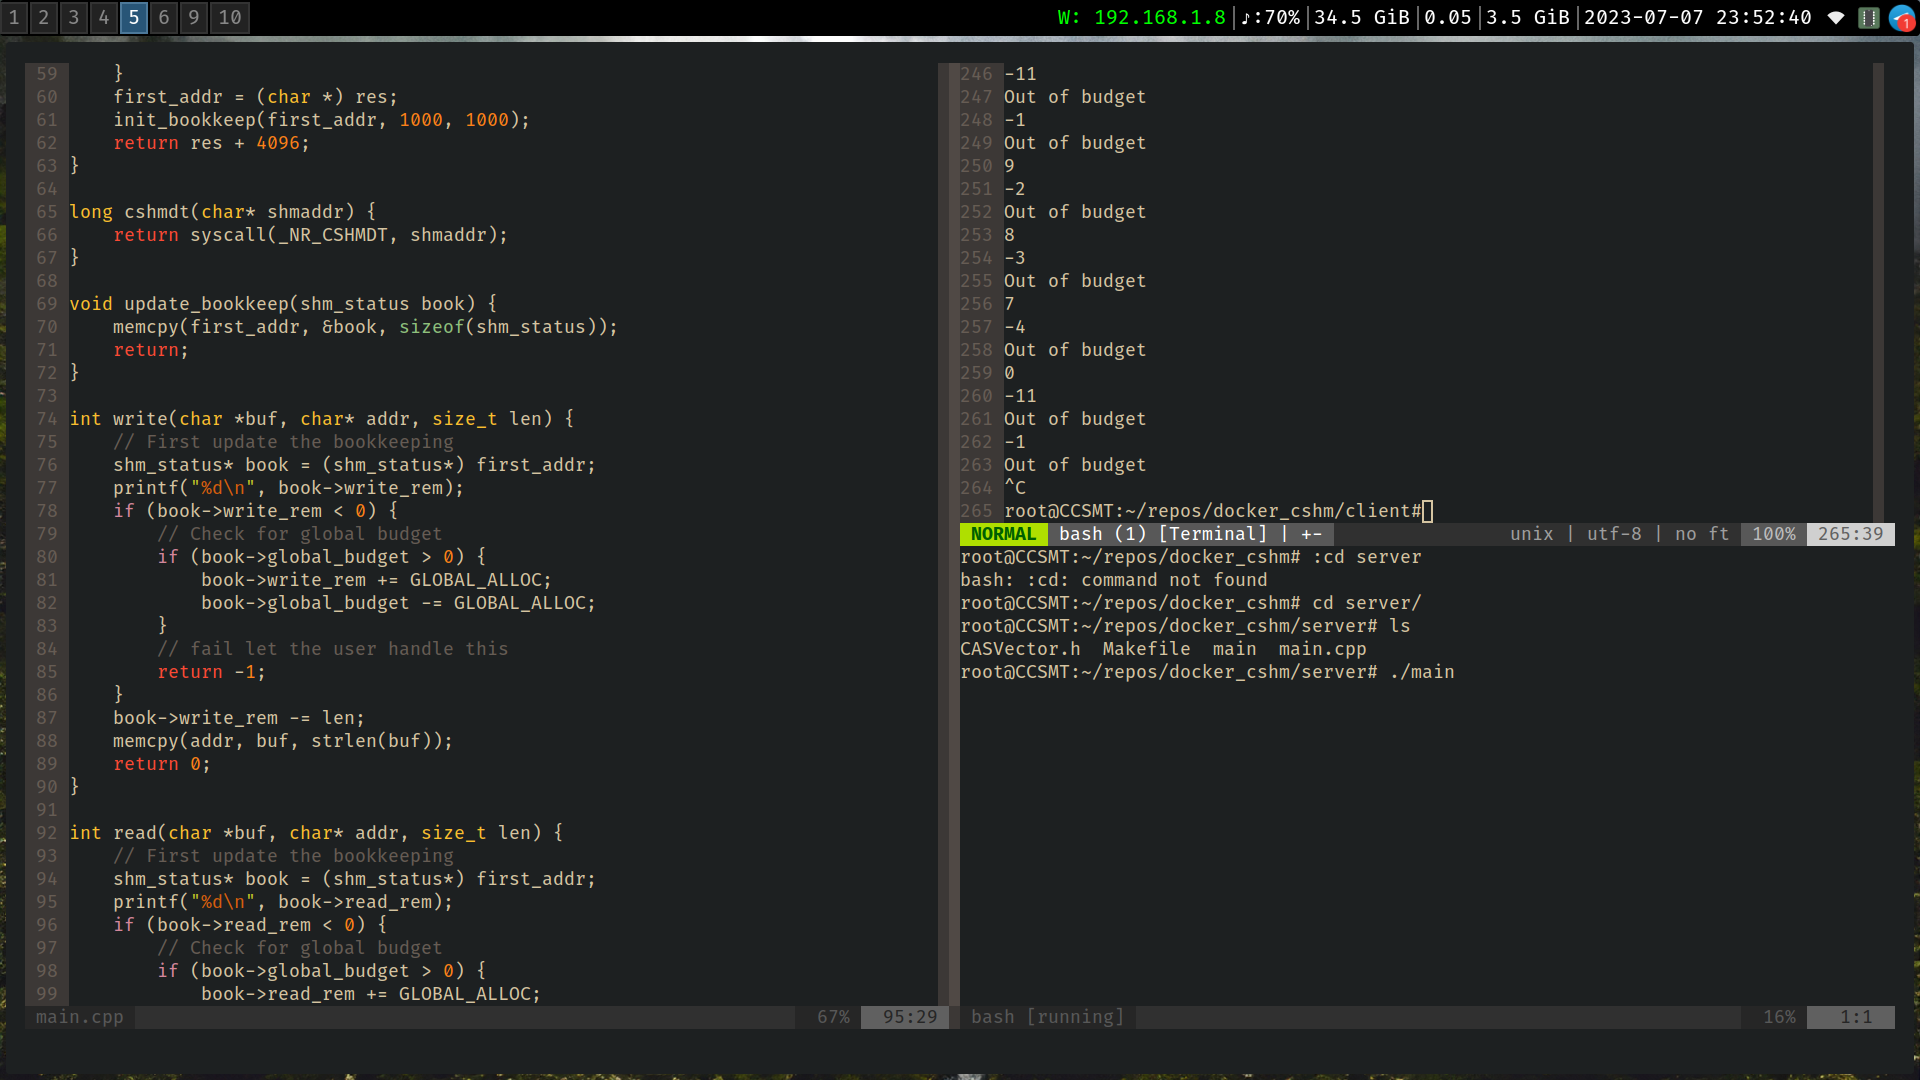
\includegraphics[scale=0.2]{results.png}
    \caption{QEMU virtual machine showing bandwidth control mechanism}
\end{figure}

In the right column, the upper pane is the client app in the docker
Every time the client is out of budget it sleeps for 1 second.
The bottom panel is the server which resets the bookkeeping at the end of the
hyper-period showing that our solution works and redistributes the budget among
the others. The result is just showing that this solution works. It could be
better to devise test cases for different scenarios but our team was unable
to meet the deadlines associated with that and was content with a working
solution.


\section{Conclusion}
In this project, we designed and implemented a bandwidth controlled shared memory
communication model for containers. Our goal was to tackle two problems in this
area.
\begin{itemize}
    \item Lack of a real-time communication method.
    \item Isolation for mixed-criticality containers.
\end{itemize}
Also with the growth of industry 4.0 the need for a real-time
virtualization solution is needed to consolidate the ECUs and small embedded
systems in these factories. By choosing containers we can lower the overhead
of the virtualization in Industry 4.0. \\
Our implementation is presented by the following codes and artifacts:
\begin{itemize}
    \item \textbf{Linux Kernel Patch:} We devised a linux kernel patch that
        edits the linux kernel and supplies us with the required system calls.
    \item \textbf{Linux Kernel Configuration:} We detected and recognized the
    required features that are needed to enable docker and containers
    functionality in linux kernel.
    \item \textbf{Compare and Swap Dynamically Allocated Atomic Vector:}
    We implemented an atomic vector according to the \cite{vector} and used
    it to eliminate contention in the shared memory space and fixed
    critical race and priority inversion bugs that are associated with
    using a mutex.
    \item \textbf{Client and Server That Implement the Bandwidth Control
        Algorthims:} We implemented these programs using C++ and used it to
        verify the bandwidth control of the shared memory subsystems.
\end{itemize}
All artifacts and source codes are presented in a zip file with this report.
Future work involving this project could be categorized as follow:
\begin{itemize}
    \item Using cache coloring and DRAM ranks to achieve hard read and write
        latency bounds.
    \item Remove the kernel patch completely or make it into a kernel module
        at most.
    \item Add an schedulability test to the shared memory for use in a container
        orchestrization tool.
    \item Use Remote Direct Memory Access to remove our local communication
        constraint.
    \item Compare RDMA and gRPC for perfomance gains and latency and in the end
        real-time capabilities.
\end{itemize}




% \bibliographystyle{abbrv}
% \bibliography{references}  % need to put bibtex references in references.bib 

\begin{thebibliography}{2}
    \bibitem{shimmy} Abranches, Marcelo, and Sepideh Goodarzy.
        "Shimmy: Shared memory channels for high performance inter-container
        communication." USENIX Workshop on Hot Topics in Edge Computing
        (HotEdge). 2019.
    \bibitem{mcs}
        Barletta, Marco, et al. "Achieving isolation in mixed-criticality
        industrial edge systems with real-time containers." 34th Euromicro
        Conference on Real-Time Systems (ECRTS 2022). Schloss
        Dagstuhl-Leibniz-Zentrum für Informatik, 2022.
    \bibitem{survey}
        Struhár, Václav, et al. "Real-time containers: A survey."
        2nd Workshop on Fog Computing and the IoT (Fog-IoT 2020).
        Schloss Dagstuhl-Leibniz-Zentrum für Informatik, 2020.
    \bibitem{memguard}
        Yun, Heechul, et al.
        "Memguard: Memory bandwidth reservation system
        for efficient performance isolation in multi-core
        platforms." 2013 IEEE 19th Real-Time and Embedded
        Technology and Applications Symposium (RTAS). IEEE, 2013.
    \bibitem{vector}
        Dechev, Damian, Peter Pirkelbauer, and Bjarne Stroustrup.
        "Lock-free dynamically resizable arrays."
        Principles of Distributed Systems: 10th International Conference,
        OPODIS 2006, Bordeaux, France, December 12-15, 2006. Proceedings 10.
        Springer Berlin Heidelberg, 2006.
\end{thebibliography}
\end{document}
